\section{Pattern und Konzepte für Resilienz in verteilten Systemen}

(Begriffe und Definitionen)

As noted in the introduction, the ``\verb|acmart|'' document class can
be used to prepare many different kinds of documentation --- a
dual-anonymous initial submission of a full-length technical paper, a
two-page SIGGRAPH Emerging Technologies abstract, a ``camera-ready''
journal article, a SIGCHI Extended Abstract, and more --- all by
selecting the appropriate {\itshape template style} and {\itshape
  template parameters}.

This document will explain the major features of the document
class. For further information, the {\itshape \LaTeX\ User's Guide} is
available from
\url{https://www.acm.org/publications/proceedings-template}.

\subsection{Circuit-Breaker}


Circuit-Breaker sind Entwurfsmuster, die dazu dienen, Fehler in verteilten Systemen zu isolieren,
indem sie den Zugriff auf fehlerhafte Dienste vorübergehend blockieren,
um eine Überlastung zu verhindern und die Systemstabilität zu gewährleisten.

\citet{Montesi.19.09.2016} heben die Rolle von Circuit-Breaker in Microservices-Architekturen hervor,
um kaskadierende Fehler zu vermeiden. % TODO "and" --> "und"
Microservices sind autonome Dienste, die über Message Passing kommunizieren, % Was ist Message Passing?
während bei \textit{Serviceorientierter Architektur} (SOA) die Komponenten einer Anwendung Teil eines
einzigen ausführbaren Artefakts, eines Monolithen, sind.

Die Hauptvorteile der \textit{Microservices-Architektur} (MSA) bestehen darin,
dass Komponenten unabhängig voneinander bereitgestellt und verwaltet werden können,
dass neue Versionen schrittweise eingeführt werden können, dass Komponenten
mithilfe verschiedener Technologien spezialisiert werden können und dass die Skalierung
effizienter durchgeführt werden kann.
Der hohe Verteilungsgrad der MSA bringt jedoch auch einige Herausforderungen mit sich,
wie z.B.\ Kommunikationsausfälle, die Überlastung von Diensten und die Notwendigkeit,
Änderungen an Dienst-APIs im Laufe der Zeit zu bewältigen.

Ein Ausfall in einer MSA gilt als unvermeidlich und kann
sich auf andere Dienste auswirken, die von dem ausgefallenen Dienst abhängig sind~\cite{Haley.28.06.2018,Montesi.19.09.2016}.
Es entsteht das Konzept des kaskadierenden Ausfalls, bei dem der Ausfall eines Dienstes
zu einem Dominoeffekt führen kann, der andere miteinander verbundene Dienste ebenfalls in
Mitleidenschaft zieht.
Um dieses Problem zu entschärfen, wird das Circuit-Breaker-Muster als Präventivmaßnahme eingeführt,
um Ausfälle innerhalb einer einzelnen Komponente einzudämmen und systemweite Ausfälle zu verhindern.
Der Grundgedanke hinter dem Circuit-Breaker-Pattern ist „Fail Fast“, d.h.\ sobald ein Dienst Anzeichen % TODO Anführungszeichen
von Unreaktivität zeigt, sollten die Anrufer sofort aufhören, auf ihn zu warten,
und die Situation in der Annahme behandeln, dass der Dienst möglicherweise nicht verfügbar ist.

Circuit-Breaker spielen eine entscheidende Rolle bei der Verbesserung der Stabilität und
Belastbarkeit von Diensten innerhalb einer MSA\@.
Clients sind in der Lage, die Verschwendung von Ressourcen für nicht reagierende Dienste zu vermeiden,
indem sie Fehler schnell erkennen und ihre Aktionen entsprechend anpassen.
Gleichzeitig wird überlasteten Diensten die Möglichkeit gegeben, sich zu erholen,
indem sie laufende Aufgaben abschließen, ohne mit weiteren Anfragen bombardiert zu werden.
Die praktische Umsetzung eines Circuit Breakers beinhaltet die Überwachung der Ausfallraten von Anrufen,
die an einen bestimmten Dienst gerichtet sind.
Wenn der Dienst Leistungsprobleme wie langsame Antworten oder häufige Fehler aufweist,
wird der Circuit-Breaker-Mechanismus ausgelöst,
sodass zukünftige Aufrufe sofort eine Fehlerantwort zurückgeben.

Das Circuit-Breaker-Muster lässt sich als endliche Maschine mit verschiedenen Zuständen
und Übergängen darstellen, die durch eine Reihe von Parametern in einer Steuertabelle gesteuert werden.
Durch die Nutzung des Leistungsschaltermusters werden die Zuverlässigkeit der Dienste und die
Ausfallsicherheit des Systems in einer MSA-Umgebung erheblich verbessert.
Dieser proaktive Ansatz schützt nicht nur vor kaskadierenden Ausfällen,
sondern gewährleistet auch eine effiziente Ressourcennutzung und fördert den allgemeinen Zustand
der miteinander verbundenen Dienste.


\paragraph{Deployment}

In diesem Paper werden drei verschiedene Ansätze für die Implementierung von Circuit-Breaker
in einer MSA diskutiert.

Der Circuit-Breaker wird in der Regel innerhalb der \textbf{Clients} eingesetzt,
wo er Aufrufe an externe Dienste abfängt.
Diese Strategie verhindert, dass Nachrichten den Zieldienst erreichen, wenn der
Leistungsschalter geöffnet ist, wodurch die Notwendigkeit ähnlicher
Schutzmechanismen im Dienst entfällt.
Allerdings beruht dieser Ansatz auf der Annahme, dass Clients zur Verwendung der Circuit Breaker
gezwungen werden können und dass sie nicht böswillig sind.
Der Nachteil besteht darin, dass das Verfügbarkeitswissen eines Dienstes auf den Client beschränkt ist,
sodass regelmäßige Pings erforderlich sind, um den Dienstintegritätsstatus abzufragen.

Eine alternative Implementierungsstrategie besteht darin,
Circuit-Breaker auf der Seite der \textbf{Dienste} oder in \textbf{Proxys} zwischen Kunden und Diensten einzuführen.
Dieser Ansatz hat seine eigenen Vor- und Nachteile.
Wenn der Circuit-Breaker auf der Seite des Dienstes platziert ist,
kann er den Dienst davor schützen, durch fehlgeschlagene Anfragen von mehreren Clients überfordert zu werden.
Außerdem hat der dienstseitige Circuit-Breaker einen globalen Überblick über die Verfügbarkeit des Dienstes,
im Gegensatz zu den client-seitigen Circuit-Breaker, die einen lokalen Überblick
auf der Grundlage der Interaktionen einzelner Clients haben.

Die Platzierung von Circuit-Breaker in Proxys zwischen Clients und Diensten
kann einen Mittelweg darstellen,
bei dem der Proxy die Kommunikation zwischen Clients und Diensten überwachen und steuern kann.
Dieser Proxy enthält für jedes Client-Dienst-Paar einen separaten Circuit-Breaker, der Anfragen nur dann zulässt,
wenn sowohl der Client- als auch der Dienst-Circuit-Breaker geschlossen sind.
Dieser Ansatz hat den Vorteil, dass keine Änderungen am Client- oder Dienstcode erforderlich sind,
da der Proxy unabhängig konfiguriert werden kann.
Außerdem schützt er sowohl Clients als auch Dienste, indem er Dienste vor zu aggressiven Clients und Clients
vor fehlerhaften Diensten abschirmt.
Allerdings führt der Proxy zu einem potenziellen Engpass im Netzwerk,
der möglicherweise durch den Einsatz mehrerer Proxys behoben werden muss.

\citet{Montesi.19.09.2016} schlagen vor, dass praktische Anwendungen diese verschiedenen Einsatzstrategien
kombinieren sollten, um die besten Ergebnisse zu erzielen.
Durch die Verwendung einer Kombination aus clientseitigen, dienstseitigen und proxy-basierten Circuit-Breaker
kann die Anwendung von den Vorteilen jedes Ansatzes profitieren und ihre jeweiligen Nachteile abmildern.
Diese Flexibilität bei der Bereitstellung ermöglicht eine robustere und effektivere Implementierung von Circuit-Breaker,
die die allgemeine Ausfallsicherheit und Verfügbarkeit des Systems verbessern kann.

Insgesamt bieten die drei vorgestellten Ansätze unterschiedliche Kompromisse in Bezug auf die Komplexität der Implementierung,
die Ressourcennutzung und den Grad des Schutzes, der den Clients und Diensten geboten wird.

\paragraph{Implementation}


Eine der bekanntesten Implementierungen von Circuit-Breaker ist die Hystrix-Bibliothek für Java,
während die Python-Bibliothek \textit{pybreaker} eine ähnliche Funktionalität bietet.
\textit{Pybreaker} ist eine flexible und leichtgewichtige Bibliothek, die es ermöglicht,
Python-Code in eine Prozedur zu verpacken, die von einem Circuit-Breaker gesteuert wird.
Diese Bibliothek hilft, den Ausfall von abhängigen Diensten oder Komponenten durch Überlastung
oder Fehler zu vermeiden und unterstützt Funktionen wie Fehlerzählung,
Zustandsüberwachung und benutzerdefinierte Rückfallstrategien. % Quelle?
\textit{Pybreaker} unterstützt sowohl Client- als auch dienstseitige Circuit-Breaker.

\tikzset{cross/.style={cross out, draw=black,thick, minimum size=10*(#1-\pgflinewidth), inner sep=1pt, outer sep=1pt,
    color=red, minimum height = 0.4cm},
%default radius will be 1pt.
cross/.default={1pt}}
\begin{figure}
\pgfdeclarelayer{background}
\pgfdeclarelayer{foreground}
\pgfsetlayers{background,main,foreground}
% Define a few styles and constants
\tikzstyle{state} = [draw, rounded corners,
text centered, minimum height=3em, minimum width=4em]
\centering
\centering
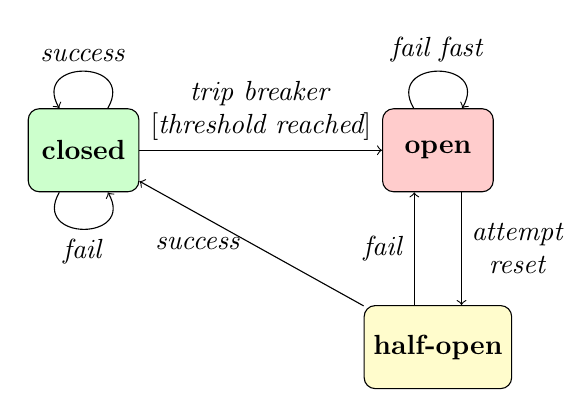
\begin{tikzpicture}[
%scale=0.6, every node/.style={scale=0.6}
]
\node (closed) [state, fill=green!20] {\textbf{closed}};
\node (open) [state, fill=red!20, right of=closed, node distance =4.5cm] {\textbf{open}};
\node (halfopen) [state, fill=yellow!20, below of=open, node distance =2.5cm] {\textbf{half-open}};
\draw [->] (closed) -- (open) node[above,midway,align=center] {\textit{trip breaker}\\\textit{$[$threshold
reached$]$}};
\draw [->] (halfopen) -- (closed) node[left,midway] {\textit{success}};
\draw [transform canvas={xshift=-0.3cm},->] (halfopen) -- (open) node[left,midway] {\textit{fail}};
\draw [transform canvas={xshift=0.3cm},->] (open) -- (halfopen) node[right,midway,align=center]
{\textit{attempt}\\\textit{reset}};
\path[]	(open)   edge[loop, in=60,out=120, looseness=3,->] node[above]  {\textit{fail fast}} (open);
\path[]	(closed)   edge[loop, in=60,out=120, looseness=3,<-] node[above]  {\textit{success}} (closed);
\path[]	(closed)   edge[loop, in=240,out=300, looseness=3,<-] node[below]  {\textit{fail}} (closed);
\end{tikzpicture}
\caption{Circuit Breaker Zustandsdiagramm nach~\cite{Montesi.19.09.2016}.}
\label{cb-fsm}
\Description{Circuit Breaker Zustandsdiagramm: closed/open/half-open}
\end{figure}

Je nach Zustand (geschlossen, offen oder halboffen) werden unterschiedliche
Aktionen ausgeführt, z.B.\ das Weiterleiten von Nachrichten, die
Behandlung von Fehlern oder das Blockieren von Anfragen, siehe Abbildung~\ref{cb-fsm}.


\subsection{Template Parameters}

In addition to specifying the {\itshape template style} to be used in
formatting your work, there are a number of {\itshape template parameters}
which modify some part of the applied template style. A complete list
of these parameters can be found in the {\itshape \LaTeX\ User's Guide.}

Frequently-used parameters, or combinations of parameters, include:
\begin{itemize}
\item {\verb|anonymous,review|}: Suitable for a ``dual-anonymous''
  conference submission. Anonymizes the work and includes line
  numbers. Use with the \verb|\acmSubmissionID| command to print the
  submission's unique ID on each page of the work.
\item{\verb|authorversion|}: Produces a version of the work suitable
  for posting by the author.
\item{\verb|screen|}: Produces colored hyperlinks.
\end{itemize}

This document uses the following string as the first command in the
source file:
\begin{verbatim}
\documentclass[acmtog]{acmart}
\end{verbatim}
